Our experimental investigation is structured into two primary focuses:

\begin{enumerate}
    \item \textbf{Reconstruction Analysis}: This part of the experiment focuses on assessing the ability of our models to accurately reconstruct time series data. The effectiveness of the reconstruction process is a crucial indicator of the model's understanding and representation of the input data. 
    \item \textbf{Representation Learning Evaluation}: The second aspect of our experiment delves into the quality of the learned representations in the discrete latent space. Here, we aim to examine the intricacies of how the models, especially our modified version, encode and represent the time series data in the latent space. 
\end{enumerate}
As a benchmark for comparison, we establish the naive VQVAE as the baseline model. Against this baseline, we examine the performance of the Barlow Twins modified VQVAE (BT-VQVAE). 
We examine how the BT-VQVAE performs as a function of $\gamma$ in eq \ref{eq:BTVQVAEloss}.  
The comparison is geared towards understanding the enhancements and differences brought about by the Barlow Twins modification, particularly in terms of the quality of the latent representations and the reconstruction accuracy.

\section{UCR Archive}
Our experiments are conducted using the UCR Archive \cite{UCRArchive2018}, a widely-used open-source repository of time series datasets. The UCR Archive contains a diverse range of time series data, including various domains and characteristics, making it a good benchmark for evaluating time series models.
The datasets in UCR Archive are divided into a training dataset aswell as a test dataset. In the experiment we train the models on the provided training dataset and validate on the test set.
The chosen subset for the experiment emphasize datasets that vary not only in size but also in the complexity and nature of their class distributions. The chosen subset also contains datasets with the highest number of samples, as done by Lee et al in their investigation of various SSL algorithms on the UCR Archive\cite{SSLs}.

\begin{table}[h]
    \centering
    \begin{tabular}{l c c r}
    \hline
    Dataset Name & \#Samples & \#Classes & Length \\
    \hline
    Electric Devices & 16637 & 7 & 46 \\
    StarLightCurves & 9236 & 3 & 1024 \\
    Wafer & 7164 & 2 & 152\\
    ECG5000 & 5000 & 5 & 140 \\
    TwoPatterns & 5000 & 4 & 128 \\
    FordA & 4921 & 2 & 500 \\
    UWaveGestureLibraryAll & 4478 & 8 & 945 \\
    FordB & 4446 & 2 & 500 \\
    ChlorineConcentration & 4307 & 3 & 166
    \end{tabular}
    \caption{Chosen UCR Archive subset. Data collected by Lee et al\cite{SSLs}}
    \label{tab:sample_table}
\end{table}

\section{Reconstruction evaluation}
We evaluate the reconstruction accuracy by calculating $\mathcal{L}_\text{recon}$ in eq \ref{eq:recon} using the validation set. 
Giving $\mathcal{L}_\text{val-recon}$.
This gives us a score on how well the models generalize on the validation set.

\section{Downstream evaluation}
In the training phase of our models, we incorporate a set of downstream tasks. These tasks are distinct from the primary training process in that they do not influence the gradient updates during backpropagation. Instead, their primary role is to offer insights into various aspects of the model's performance and capabilities.

In our case, we are interested in how the fundamental structure of the discrete latent space change during training for the two models. Aswell as how the different types of timeseries are ordered spacially as discrete latent representations. 

\subsection{Extracting Discrete latent variables}
The UCR archive include labels $Y$ alongside the set of timeseries $X$. Splitted in training and validation datasets respectively. The process of extracting the latent representations is by propagating $X_\text{train}$ and $X_\text{test}$ through the encoder and quantization model seperatively. 
This gives us the models discrete latent representations, $Z_\text{train}$ and $Z_\text{test}$, as illustrated in fig \ref{fig:latents}. The concatenation of $Z_\text{train}$ and $Z_\text{test}$ is denoted as $Z$.

\begin{figure}[H]
    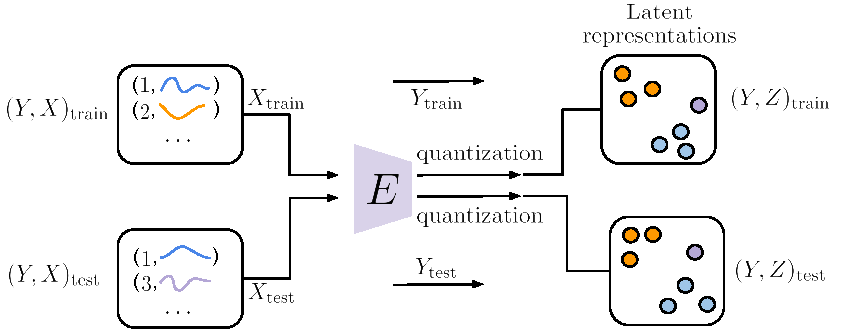
\includegraphics[scale=0.8]{figures/figure-pdf/Downstreams.pdf}
    \caption{Illustration showing the processing of training and validation datasets to latent representations.}
    \label{fig:latents}
\end{figure}

This gives us the encoder-codebook latent representations, which is usefull to examine how the 

\subsection{Downstream tests}
The \textbf{intrinstic dimension} measure identifies the most straight forward yet comprehensive set of features required to grasp our data's structure. We approximate the intrinstic dimension by applying a Principal Component Analysis (PCA) on $Z$ and pinpoint the number of principal components that account for 95\%
of the variance. This provides a measure of the complexity of the discrete latent variables. 

By fitting supervised models on $(Z, Y)_\text{train}$ and predicting on $(Z, Y)_\text{test}$ we can investigate the richness of information in the discrete latent variables related to the labels.
We use two supervised approaches: \textbf{SVM} and \textbf{KNN}. The SVM is implemented with a linear kernel, hence measuring the linear seperatability of the latent space. A high classification accuracy would suggest that the labeled timeseries are linearly separable as discrete latent representations. 
For the KNN algorithm we experiment with three different values for K, namely $1, 5, 10$. The intuition being that a high accuracy with a $K=1$ would suggest more complexity, compared to a high accuracy with $K=10$.

Additionally to the richness of information related to the labels, we are also investigating if the discrete latent variables ($Z_\text{train}$, $Z_\text{test}$) are seperatable into clusters. We test this by designing a experiment using the unsupervised \textbf{KMeans} algorithm and \textbf{Silhouette score}.
By fitting 15 Kmeans clusters on the latent representations  and average the silhouette scores, we get a downstream metric of how well the discrete latent space is clusterable for each model. 

